%% ---------------------------------------------------------------------------
%%  UnionLabs — demo talk slides, built from the MobiCom demo paper.
%%  Same figures (figs/*.pdf), same palette (unionstyle colours).
%%  Build:  pdflatex unionlabs-slides.tex   (twice, for nav dots)
%% ---------------------------------------------------------------------------
\documentclass[aspectratio=169,10pt]{beamer}
\usepackage{graphicx}
\graphicspath{{figs/}}

%% ── the UnionLabs palette (mirrors figs/unionstyle.tex) ──
\definecolor{uCode}{HTML}{1F6F5C}
\definecolor{uApi}{HTML}{6B4BA8}
\definecolor{uPhy}{HTML}{2E5E9E}
\definecolor{uRadio}{HTML}{B4700F}
\definecolor{uShare}{HTML}{8A2E4D}

%% ── a quiet theme ──
\usetheme{default}
\usecolortheme{seagull}
\setbeamercolor{structure}{fg=uApi}
\setbeamercolor{frametitle}{fg=uApi,bg=white}
\setbeamerfont{frametitle}{series=\bfseries,size=\large}
\setbeamercolor{title}{fg=uApi}
\setbeamertemplate{navigation symbols}{}
\setbeamertemplate{footline}[frame number]
\setbeamertemplate{itemize items}[circle]
\setbeamercolor{itemize item}{fg=uApi}
\setbeamercolor{itemize subitem}{fg=uPhy}
\newcommand{\mono}[1]{{\ttfamily\small #1}}

\title{\textbf{UnionLabs: new agent, features, physical layers}}
\author{First Author \and Second Author \and Third Author\\[2pt]
  {\small Institution}}
\date{ACM MobiCom '26 Demo \,·\, Austin, TX \,·\, October 2026}

\begin{document}

%% ── 1 · title ─────────────────────────────────────────────────────────────
\begin{frame}
  \titlepage
\end{frame}

%% ── 2 · motivation ────────────────────────────────────────────────────────
\begin{frame}{The problem: everything \emph{around} the algorithm}
  \begin{itemize}\setlength\itemsep{0.7em}
    \item A learning-over-radio experiment is easy to state and expensive to
      run --- the algorithm is a page of code; what surrounds it is not.
    \item Platforms removed the hardware barrier, open stacks the waveform
      barrier \dots
    \item \dots but users still hand-link algorithms to the physical layer:
      hundreds of lines, days of debugging.
    \item The wiring lives in operators' heads and shell history --- retyped
      per machine, and the retypings disagree.
  \end{itemize}
  \vspace{1em}
  \centering
  {\color{uShare}\bfseries UnionLabs separates \emph{what an algorithm does}
   from \emph{how the experiment is wired}.}
\end{frame}

%% ── 3 · the four parts ────────────────────────────────────────────────────
\begin{frame}{Four designed parts}
  \begin{columns}[T]
    \column{0.5\textwidth}
      \begin{itemize}\setlength\itemsep{0.9em}
        \item {\color{uApi}\textbf{The Agent}} --- any machine becomes a
          managed edge node
        \item {\color{uShare}\textbf{The shared workspace}} --- one account's
          state, across testbeds
        \item {\color{uCode}\textbf{The algorithm contract}} ---
          \mono{transmit()} / \mono{receive(msg)}, nothing else
        \item {\color{uPhy}\textbf{The PHY codes}} --- a modem whose every
          stage is selectable
      \end{itemize}
    \column{0.45\textwidth}
      \centering
      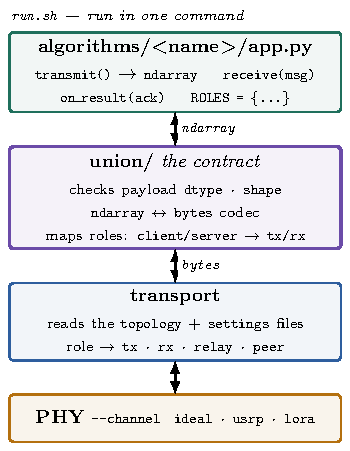
\includegraphics[height=0.78\textheight]{fig-union-api-col}
  \end{columns}
\end{frame}

%% ── 4 · agent ─────────────────────────────────────────────────────────────
\begin{frame}{The UnionLabs Agent}
  \begin{columns}[T]
    \column{0.5\textwidth}
      \begin{itemize}\setlength\itemsep{0.7em}
        \item One agent per edge node --- server, workstation, or laptop.
        \item Install: prepares AWS, Docker, RKE2, Helm; registers with a
          unique edge ID + token.
        \item gRPC with the cloud: instructions down, status + heartbeats up.
        \item Owner uploads the topology via the visualizer; reservation
          allocates from it --- live nodes only.
        \item Experiments become Kubernetes pods; devices exposed
          \emph{only by the owner's permission}.
        \item Remote access rides the cloud--edge path: pods never publicly
          exposed.
      \end{itemize}
    \column{0.44\textwidth}
      \centering
      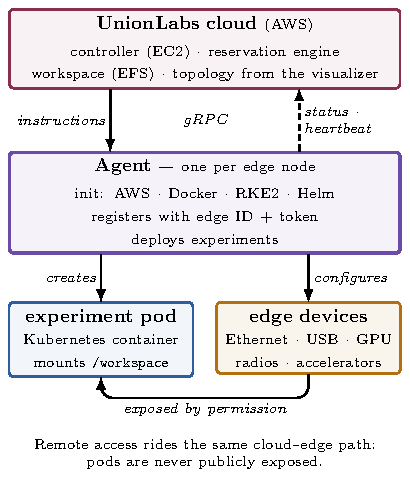
\includegraphics[height=0.8\textheight]{fig-agent-col}
  \end{columns}
\end{frame}

%% ── 5 · workspace ─────────────────────────────────────────────────────────
\begin{frame}{One workspace across testbeds}
  \begin{columns}[T]
    \column{0.5\textwidth}
      \begin{itemize}\setlength\itemsep{0.7em}
        \item Every session of an account mounts the same
          \mono{/workspace} --- even when the testbeds cannot reach each
          other.
        \item \mono{topologies/}: authored wiring, written once.
        \item \mono{settings/}: each session's own record --- 30\,s
          heartbeat, dropped when stale.
        \item Two kinds of state, two lifecycles: the shared file system
          never carries a fact that can go stale.
      \end{itemize}
    \column{0.44\textwidth}
      \centering
      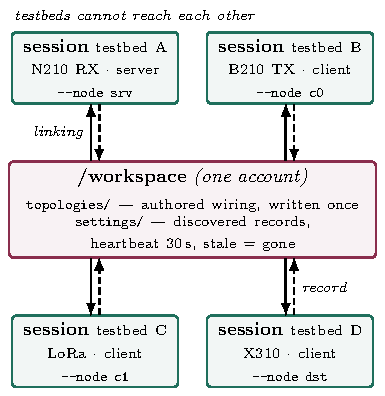
\includegraphics[width=\linewidth]{fig-shared-workspace-col}
  \end{columns}
\end{frame}

%% ── 6 · contract ──────────────────────────────────────────────────────────
\begin{frame}{The algorithm contract --- \mono{run.sh}, one command}
  \begin{columns}[T]
    \column{0.5\textwidth}
      \begin{itemize}\setlength\itemsep{0.7em}
        \item The algorithm writes \mono{transmit()} and
          \mono{receive(msg)} --- and imports nothing from any radio driver.
        \item The union layer validates payloads, converts
          \mono{ndarray} $\leftrightarrow$ bytes, maps role names.
        \item The transport reads the topology + settings files; the node
          becomes \mono{tx · rx · relay · peer}.
        \item \mono{-{}-channel} selects the PHY: \mono{ideal · usrp · lora}.
        \item Same path, both directions --- change the physical layer with
          one flag, no code change.
      \end{itemize}
    \column{0.44\textwidth}
      \centering
      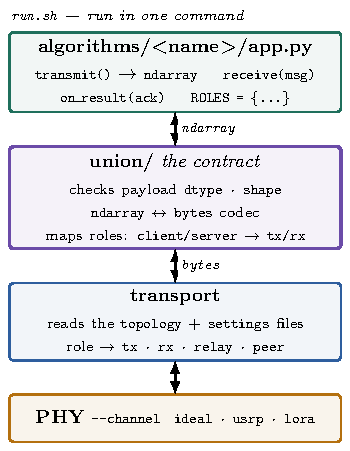
\includegraphics[height=0.8\textheight]{fig-union-api-col}
  \end{columns}
\end{frame}

%% ── 7 · PHY ───────────────────────────────────────────────────────────────
\begin{frame}{The PHY codes}
  \centering
  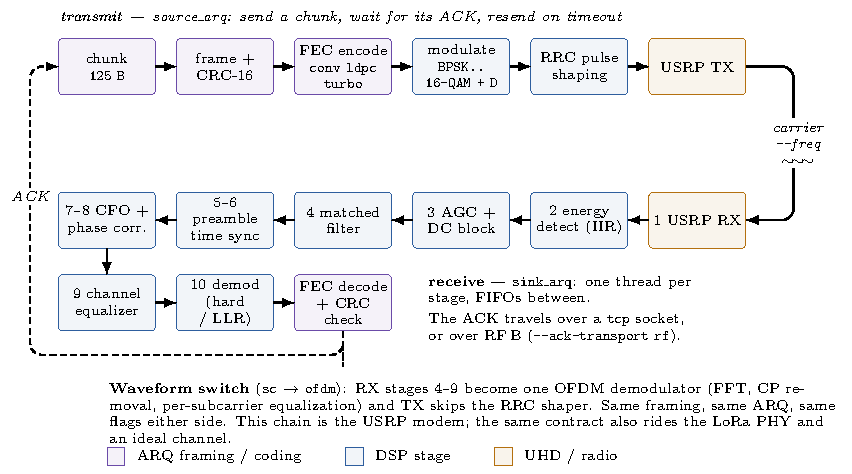
\includegraphics[width=0.74\linewidth]{fig-phy-pipeline}
  \vspace{0.4em}
  \begin{itemize}
    \item Modulation, coding, synchronization, waveform, gains, carrier ---
      all selectable per experiment.
    \item Stop-and-wait ARQ end to end; the ACK over TCP or a second RF
      path.
  \end{itemize}
\end{frame}

%% ── 8 · wiring ────────────────────────────────────────────────────────────
\begin{frame}{Wiring as a file}
  \begin{itemize}\setlength\itemsep{0.8em}
    \item A topology names each node, its role, its radio, its ports, and
      the links between nodes --- every node launches from the same file.
    \item \textbf{Per-link, per-direction media}: one hop over the air, the
      next over Ethernet; the reply may return over TCP/IP.
    \item A wiring that cannot run is \textbf{refused when it is read},
      naming the node at fault --- not minutes later, from the wrong layer.
    \item One command walks 44 flags and 82 topology settings from typed
      text to the object each configures.
  \end{itemize}
\end{frame}

%% ── 9 · demonstration ─────────────────────────────────────────────────────
\begin{frame}{Demonstration: each part, working}
  \begin{enumerate}\setlength\itemsep{0.8em}
    \item \textbf{Onboarding (Agent)} --- a machine enrolled on the spot;
      heartbeat appears; the visitor opens the container's remote desktop.
    \item \textbf{One workspace} --- edit a wiring file here, see it from a
      session on a remote testbed.
    \item \textbf{One algorithm, different PHYs} --- radio-free, then real
      radios by one flag; delivery, retransmissions, airtime on screen.
    \item \textbf{Rewiring, and refusal} --- a multi-hop experiment changes
      medium by one field; an impossible wiring is refused by name.
  \end{enumerate}
\end{frame}

%% ── 10 · takeaway ─────────────────────────────────────────────────────────
\begin{frame}{Takeaway}
  \begin{center}
    {\Large\bfseries Write the experiment once.\\[4pt]
     Run it over any PHY, topology, and testbed.}\\[1.5em]
    \mono{./run.sh -{}-algo <yours> -{}-topology <wiring> -{}-node <me>}\\[2em]
    {\color{uShare} One command · one wiring file · one contract}\\[2em]
    {\small Come run it at the table.}
  \end{center}
\end{frame}

\end{document}
